\section*{Experiment 1}

The graph for experiment 1 is shown in Fig.~\ref{fig:chart1}. Note
that I multiplied throughputs with 1000 for the sake of presentation.

\begin{figure}[!ht]
  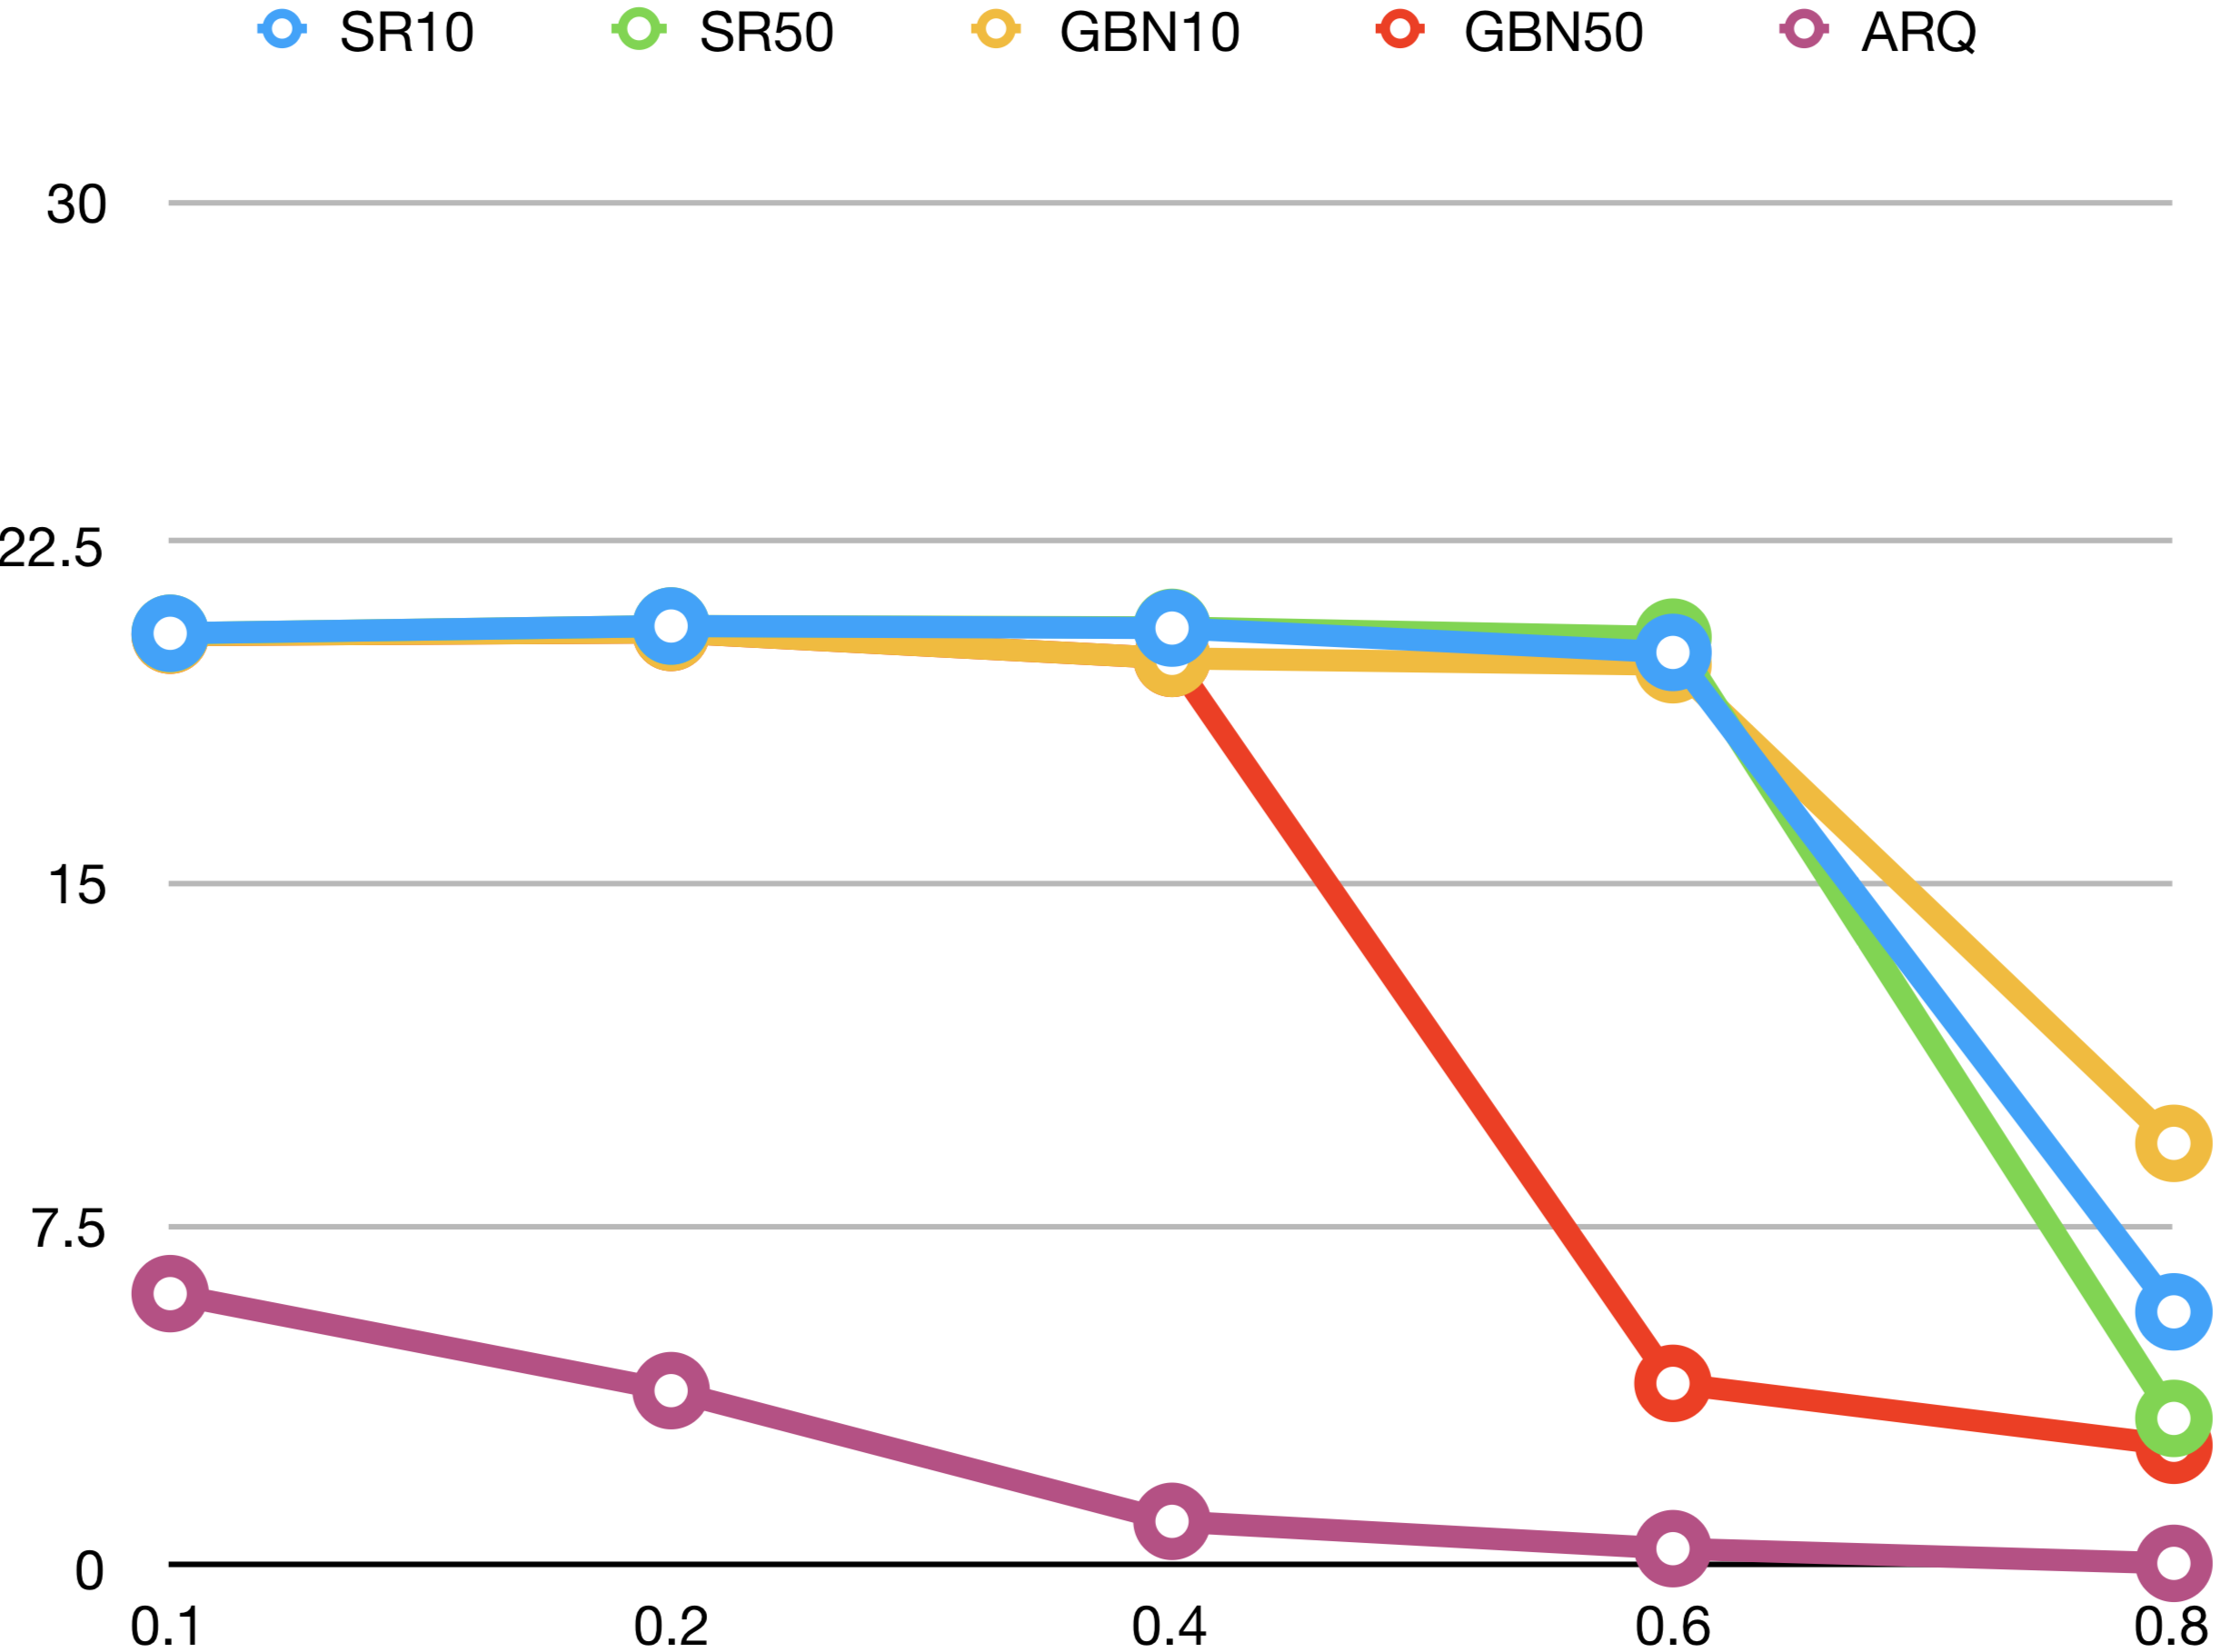
\includegraphics[width=0.8\textwidth]{chart1-fig}
  \caption{Experiment-1 data visualized. On x-axis is the loss
  probability. On y-axis is Throughput $\times$ 1000.}
  \label{fig:chart1}
\end{figure}

The raw data is shown below. Each cell has two components: the number
of messages received by layer 5, and the time it took for the
simulation to complete.
Fig.~\ref{fig:chart1}
\begin{center}
\begin{verbatim}
            0.1       0.2       0.4       0.6       0.8
----------------------------------------------------------
SR10        999       999       999        999      276
           48714     48348     48458      49749     49345

SR50        999       999       999       997       163
           48714     48348     48404      48834     49944

GBN10       999       999       998       986       462
           48824     48675     50019      49750    49655

GBN50       999       999       998       201       134
           48824     48675     50019      49864    50181

ARQ         297       196       49        26        4
           49472     50633     48570      49746     51320
\end{verbatim}
\end{center}

\paragraph{Observations}. The throughput for Selective Repeat (SR) and
Go-Back-N (GBN) is much higher than Alternating Bit Protocol (ARQ).
This is as expected.

\section*{Experiment 2}

The raw data for experiment 2 is shown below. The graph is going to be
more or less straight lines parallel to the x-axes, hence not worth
presenting.

\begin{verbatim}
          0.2           0.4
-------------------------------
SR10      999           999
          48348        48458     

SR50      999           999
         48348         48404

SR100     999           999
         48404         48404

SR200     997           999
         48348         48404

SR500     999           999
         48348         49404

GBN10     999           998
         48675         50019

GBN50     999           998
         48675         50019 

GBN100    999           998
         48675         50019 

GBN200    999           998
         48675         50019

GBN500    999           998
         48675         50019

ARQ			      196           49
				         50633         18570
\end{verbatim}

